% !TeX program = xelatex
\documentclass[aspectratio=169, 10pt]{beamer}
\usetheme{gotham}

\gothamset{
	numbering=framenumber,
	sectiontocframe default=off,
	subsectiontocframe default=off,
	parttocframe default=off,
}

% ---------------------------------------------------------------------------
% Packages
% ---------------------------------------------------------------------------
\usepackage{fontspec}
\usepackage[brazil]{babel}
\usepackage{csquotes}
\usepackage{amsmath, amssymb}
\usepackage{booktabs}
\usepackage{tikz}
\usepackage{graphicx}
\usepackage{caption}
\usepackage{moresize}
\usetikzlibrary{arrows.meta, positioning, shapes.geometric, calc}
\usepackage{listings}
\lstset{
	basicstyle=\ttfamily\scriptsize,
	keywordstyle=\bfseries,
	commentstyle=\color{gray}\itshape,
	showstringspaces=false,
	breaklines=true,
	language=Python,
}
\usepackage{appendixnumberbeamer}
\usepackage{hyperref}
\usepackage{bm}
\usepackage{float}
\usepackage{makecell}

% ---------------------------------------------------------------------------
% Bibliography (biblatex)
% ---------------------------------------------------------------------------
\usepackage[
	backend=biber,
	style=numeric,
	sorting=none,
]{biblatex}
\addbibresource{references.bib}

% ---------------------------------------------------------------------------
% Shorthands used across sections
% ---------------------------------------------------------------------------
\newcommand{\docalculus}{\emph{do}-calculus}

\newcommand{\notebooklink}[2]{%
	\centering
	\begin{center}
	\begin{beamercolorbox}[sep=10pt, rounded=true, center, shadow=false, wd=1\textwidth]{block body}
		\centering 
		{\Large \textbf{Mão na massa! $\rightarrow$  Notebook #1}}
		\\[20pt]
		\normalsize\texttt{#2}
	\end{beamercolorbox}
	\end{center}
}

% ---------------------------------------------------------------------------
% Front matter
% ---------------------------------------------------------------------------
\title[Causality for Data Scientists]{Causality for Data Scientists}
\subtitle{Discovery, Causal Inference, and Applications in Machine Learning}
\date{SBBD 2026}
\author[Gustavo de Oliveira et al.]{Gustavo Ferreira Viegas de Oliveira}
\institute[UFV]{
	Universidade Federal de Viçosa (UFV) \\
	NESPeD Lab \\
	\texttt{gustavo.viegas@ufv.br}
}

\begin{document}

\input{sections/00_capa}
% Sumário -------------------------------------------------------------
\section*{Agenda}

\begin{frame}[toc]{Agenda do minicurso}
	\tableofcontents[hideallsubsections]
\end{frame}

\begin{frame}{Formato}
	\begin{center}
	\begin{tabular}{lll}
		\toprule
		\textbf{Horário} & \textbf{Bloco} & \textbf{Conteúdo} \\
		\midrule
		14h -- 16h    & Parte 1 & Fundamentos: grafos e causal discovery \\
		16h -- 16h30  & \emph{Coffee break} & \\
		16h30 -- 18h30 & Parte 2 & Causal inference e aplicações em ML \\
		\bottomrule
	\end{tabular}
	\end{center}
	\vfill
	\textbf{Utilize seu notebook!} Os exercícios rodam no Google Colab ou Jupyter Notebook.
\end{frame}

% Biografias ----------------------------------------------------------------
\section{Sobre os autores}

\begin{frame}{Quem está apresentando}
	\begin{columns}[c]
		\begin{column}{0.32\textwidth}
			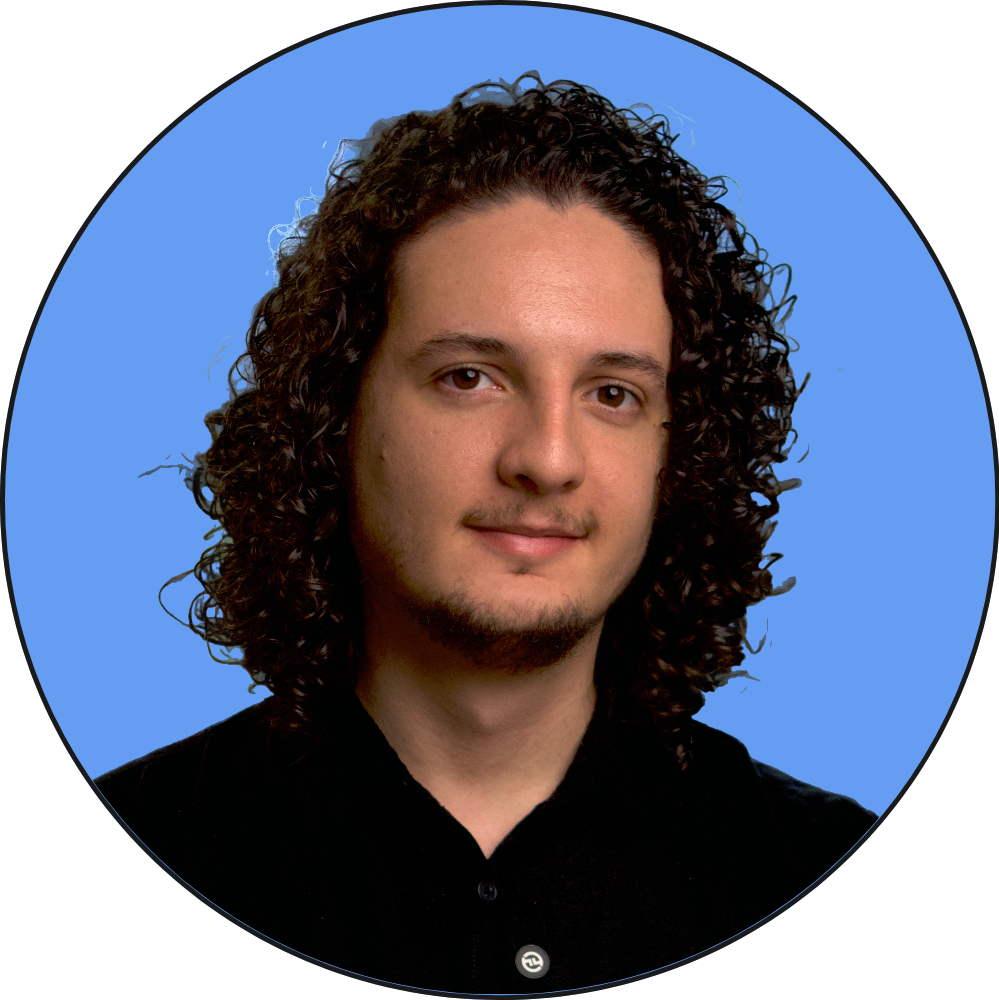
\includegraphics[width=\linewidth]{figures/gustavo_portait.png}
		\end{column}
		\begin{column}{0.66\textwidth}
			\textbf{Gustavo Ferreira Viegas de Oliveira (Apresentador)} \\
			{}
			[\href{https://lattes.cnpq.br/6788178534558304}{Lattes}]
			[\href{https://www.linkedin.com/in/gfviegas}{Linkedin}]

			\vspace{10pt}

			\small
			Bacharel e mestre em Ciência da Computação pela Universidade Federal de Viçosa (UFV). Minha dissertação
			desenvolveu o Causal-Nest (\cite{causal-nest-kbs}), framework que automatiza
			o pipeline de descoberta, estimação e refutação causal para profissionais
			de ML.
			\\ CTO e co-fundador da startup Hubs Contabilidade.
		\end{column}
	\end{columns}
\end{frame}

\begin{frame}{Orientadores}
	\textbf{Fabrício Aguiar Silva} [\href{http://lattes.cnpq.br/4039841663043863}{Lattes}]

	\small
	É doutor em Ciência da Computação pela UFMG (2015), com tese premiada
	como segunda melhor do Brasil pela SBC. Professor da UFV -- Campus Florestal
	desde 2010, atua em inteligência artificial aplicada e sistemas distribuídos.
	Orientador de mestrado do apresentador.

	\vfill
	\normalsize
	\textbf{Marcus Henrique Soares Mendes} [\href{https://lattes.cnpq.br/9729345585563115}{Lattes}]

	\small
	É doutor em Engenharia Elétrica pela UFMG (2013) e Professor Titular da
	UFV -- Campus Florestal desde 2005. Atua em otimização, computação evolutiva
	e meta-heurísticas. Co-orientador de mestrado do apresentador.
\end{frame}

% Motivação ----------------------------------------------------------
\section{Motivação}

\begin{frame}{ML é ótimo para associações}
	\textbf{ML tradicional é excelente em perguntas como:}
	\begin{center}
		\Large \emph{``O que costuma acontecer junto de X?''}
	\end{center}
	\vfill
	\pause
	Mas não é tão eficaz para perguntas do tipo:
	\begin{itemize}
		\item \textbf{``O que acontece se eu intervir?''} --- \emph{do}(X)
		\item \textbf{``Quais atributos realmente causam esse resultado?''}
		\item \textbf{``O que precisaria mudar para o resultado ser diferente?''}
	\end{itemize}
\end{frame}

\begin{frame}{Associação $\neq$ Intervenção}
	\begin{block}{Um exemplo clássico}
		Alarmes de incêndio estão fortemente correlacionados com a presença de bombeiros no local.
	\end{block}
	\pause
	\begin{alertblock}{Intervenção é outra coisa}
		Instalar mais alarmes (\emph{do}(alarme = ligado)) não traz mais bombeiros.
	\end{alertblock}
	\pause
	\centering \textbf{$P(Y \mid X) \neq P(Y \mid do(X))$}
\end{frame}

\begin{frame}{Correlação $\neq$ Causalidade}
	\centering
	{\large Nicolas Cage causa afogamentos?}
	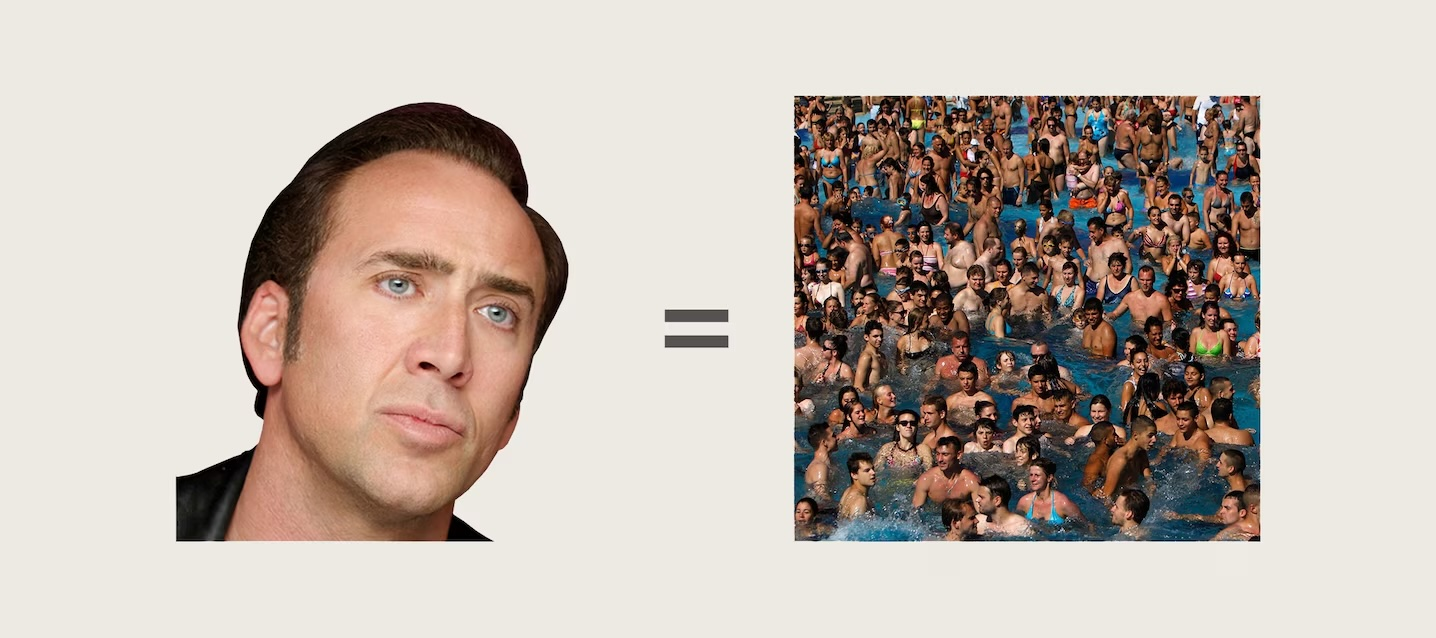
\includegraphics[width=\linewidth]{figures/nicolas_cage_drowning.jpg}
\end{frame}
\begin{frame}{Correlação $\neq$ Causalidade}
	\centering
	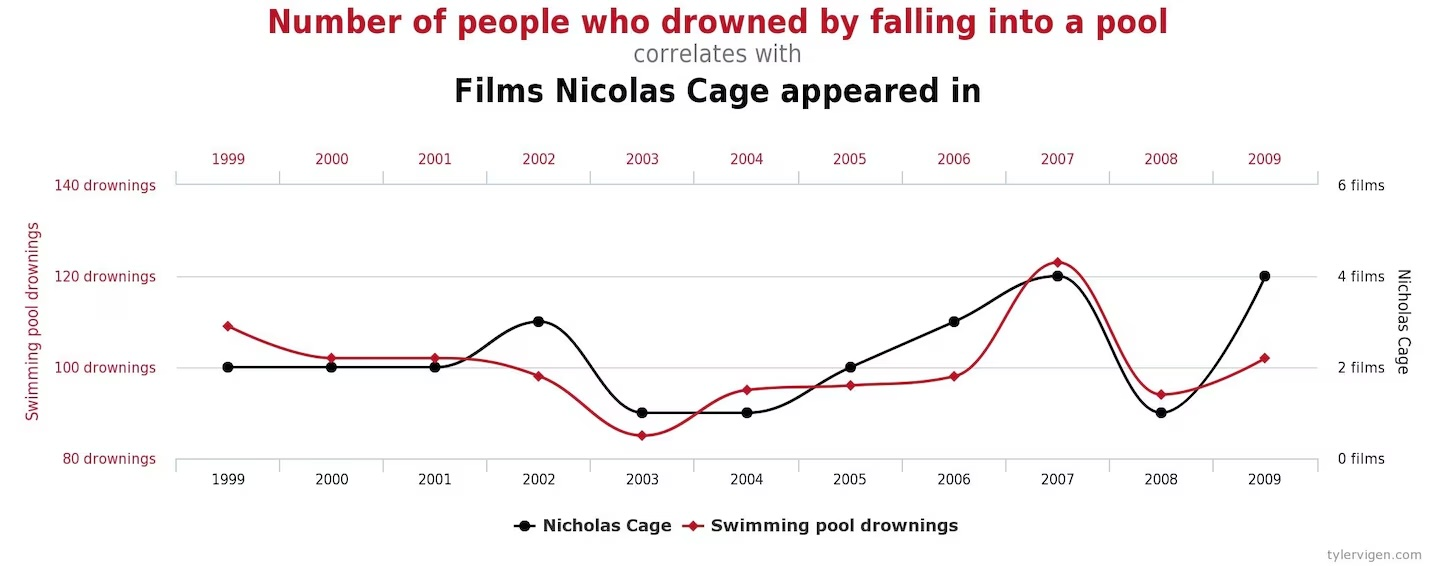
\includegraphics[width=\linewidth]{figures/nicolas_cage_drowning_2.jpg}
\end{frame}

\begin{frame}{... e o que isso tem a ver com ciência de dados?}
	Duas variáveis podem ter uma associação em um sentido na população inteira, e no sentido oposto em \emph{cada} subgrupo.
	\pause
	\vfill
	Esse cenário não é muito raro, e é consequência direta de confundimento (\emph{confounding}). 

	Vamos ver?
\end{frame}

\subsection{Paradoxo de Simpson}

% \begin{frame}{Paradoxo de Simpson}
% 	\textbf{Planejado (plan.md 4.1):}
% 	\begin{itemize}
% 		\item Limitações do ML tradicional: associação vs. intervenção
% 		\item Estudo de caso: vacinação COVID-19 (Reino Unido)
% 		\item Reversão de tendência por subgrupo (idade)
% 	\end{itemize}
% \end{frame}

\begin{frame}{Mão na massa}
	\notebooklink{1}{1\_simpsons\_paradox\_example.ipynb}
\end{frame}



\section{Causalidade}

\begin{frame}{Causalidade}
    \begin{itemize}
        \item Causalidade é a relação entre causa e efeito;
        \item Aplicações relevantes na vida real: medicina, economia, política, etc.;
        \item Interesse crescente na área de pesquisa: Airbnb, Uber, Salesforce, Microsoft...
    \end{itemize}
    \vspace{20pt}
    Adotar o estudo de causalidade permite melhorar a tomada de decisão, prever resultados de intervenções e entender relações complexas entre variáveis.
\end{frame}

\begin{frame}{Interventions e o operador \emph{do}}
    Pearl introduziu um framework formal para modelar intervenções:

    \begin{itemize}
        \item \bm{$P(Y \mid X)$} representa a probabilidade de $Y$ dado que observamos $X$;
        \item \bm{$P(Y \mid do(X))$} representa a probabilidade de $Y$ quando intervenimos para fixar $X$ em um valor específico;
    \end{itemize}

    \pause
    \begin{itemize}
        \item \bm{$P(Y \mid X)$} reflete correlações que podem resultar de múltiplos caminhos causais.
        \item \bm{$P(Y \mid do(X))$} isola o efeito causal de $X$ sobre $Y$ simulando uma intervenção que elimina influências causais à $X$.
    \end{itemize}
\end{frame}

\begin{frame}{Interventions e o operador \emph{do}}{Um exemplo...}
    \begin{itemize}
        \item \bm{$P(recuperou \mid {medicado})$} indica: \pause correlação, possivelmente confundida por fatores como idade, gravidade da doença, etc.;
        \pause
        \item \bm{$P(recuperou \mid do({medicado}))$} indica: \pause o efeito causal do remédio na recuperação, isolando o impacto de outros fatores.
    \end{itemize}

    \pause

    Podemos distinguir essas duas probabilidades coletando mais dados?
    \pause
    \centering
    
\includegraphics[width=0.3\textwidth]{figures/no.jpg}
\end{frame}
\begin{frame}{Hierarquia Causal e os limites de ML tradicional}
    \begin{center}
        \begin{tikzpicture}[
            level/.style={draw, rounded corners, minimum width=11cm, minimum height=1.55cm, align=center},
            arrow/.style={->, thick, >=stealth}
        ]
        \node[level, fill=blue!15] (l1) at (0,0) {
            \textbf{Nível 1: Associação (Observar)} \\[2pt]
            \small \textit{O que é?} \\
            \small ``O que um sintoma me diz sobre uma doença?''
        };
        \node[level, fill=orange!20] (l2) at (0,2) {
            \textbf{Nível 2: Intervenção (Agir)} \\[2pt]
            \small \textit{E se eu agir?} \\
            \small ``O que acontece se eu tomar este medicamento?''
        };
        \node[level, fill=green!20] (l3) at (0,4) {
            \textbf{Nível 3: Counterfactuals (Imaginar)} \\[2pt]
            \small \textit{Por quê? E se eu agisse de forma diferente?} \\
            \small ``Foi o medicamento que me curou?''
        };
        \draw[arrow] (l1.north) -- (l2.south);
        \draw[arrow] (l2.north) -- (l3.south);
        \node[rotate=90, anchor=center] at (-6.5,2) {\small Aumento de habilidade cognitiva};
        \end{tikzpicture}
        \label{fig:causal_hierarchy}
    \end{center}
\end{frame}

\begin{frame}{Modelos Gráficos Causais}{Grafos Acíclicos Dirigidos (DAGs)}
    \begin{columns}[T]
        \begin{column}{0.52\textwidth}
            \begin{itemize}
                \item Nós = variáveis; 
                \item Arestas dirigidas = causalidade direta;
                \item $X \rightarrow Y$: $X$ é causa direta de $Y$ %($X$ é pai de $Y$)
                \vspace{20pt}
                \item<2-> Como esses grafos são "criados"?
                \item<3-> Modelados por especialistas de negócios...
                \item<4-> ...ou descobertos a partir de algoritmos especializados (Causal Discovery).
            \end{itemize}
        \end{column}
        \begin{column}{0.44\textwidth}
            \centering
            \vspace{6pt}
            \begin{tikzpicture}[
                nd/.style={draw, circle, minimum size=0.9cm, fill=blue!10, font=\footnotesize},
                ar/.style={->, thick, >=stealth}
            ]
            \node[nd] (age)  at (1,   2)  {Idade};
            \node[nd] (edu)  at (0.3, 0.4) {Educ.};
            \node[nd] (inc)  at (2.1, 0.4) {Renda};
            \node[nd] (loan) at (3,  -1)   {Emprést.};
            \draw[ar] (age) -- (edu);
            \draw[ar] (age) -- (inc);
            \draw[ar] (edu) -- (inc);
            \draw[ar] (inc) -- (loan);
            \draw[ar] (edu) -- (loan);
            \end{tikzpicture}
            \label{fig:dag_example}
        \end{column}
    \end{columns}
\end{frame}

\begin{frame}{Modelos Gráficos Causais}{Confounders, Mediators e Colliders}
    Um \textit{confounder} é uma causa comum do tratamento \bm{$X$} e do resultado \bm{$Y$}, representado por uma bifurcação no DAG: \bm{$X \leftarrow Z \rightarrow Y$}.

    \bm{$Z$} cria uma associação espúria entre \bm{$X$} e \bm{$Y$}, mesmo que não haja relação causal direta entre eles.

    \vfill

    \begin{figure}[htbp]
        \centering
        \begin{tikzpicture}[
            gnode/.style={draw, circle, minimum size=0.85cm, font=\small},
            arrow/.style={->, thick, >=stealth}
        ]
        % --- (a) Confounder (Fork) ---
        \node[gnode] (Xf) at (0.0, 0) {$X$};
        \node[gnode] (Zf) at (1.5, 1.2) {$Z$};
        \node[gnode] (Yf) at (3.0, 0) {$Y$};
        \draw[arrow] (Zf)--(Xf);
        \draw[arrow] (Zf)--(Yf);
        \node[font=\small\bfseries] at (1.5, -0.8) {(a) Confounder};
        \node[font=\footnotesize] at (1.5, -1.25) {$X \leftarrow Z \rightarrow Y$};
        \end{tikzpicture}
        \end{figure}
\end{frame}

\begin{frame}{Modelos Gráficos Causais}{Confounders, Mediators e Colliders}
    Um \textit{mediator} é uma variável que está no caminho causal entre \bm{$X$} e \bm{$Y$}, representado por uma cadeia no DAG: \bm{$X \rightarrow M \rightarrow Y$}.

    O mediador \bm{$M$} transmite o efeito causal de \bm{$X$} para \bm{$Y$}.

    \vfill

    \begin{figure}[htbp]
        \centering
        \begin{tikzpicture}[
            gnode/.style={draw, circle, minimum size=0.85cm, font=\small},
            arrow/.style={->, thick, >=stealth}
        ]
       
        % --- (b) Mediator (Chain) ---
        \node[gnode] (Xc) at (4.5, 0) {$X$};
        \node[gnode] (Mc) at (6.0, 0) {$M$};
        \node[gnode] (Yc) at (7.5, 0) {$Y$};
        \draw[arrow] (Xc)--(Mc);
        \draw[arrow] (Mc)--(Yc);
        \node[font=\small\bfseries] at (6.0, -0.8) {(b) Mediator};
        \node[font=\footnotesize] at (6.0, -1.25) {$X \rightarrow M \rightarrow Y$};

        \end{tikzpicture}
        \end{figure}
\end{frame}

\begin{frame}{Modelos Gráficos Causais}{Confounders, Mediators e Colliders}
    Um \textit{collider} é uma variável que é causada por outras duas variáveis, representado por uma estrutura em "V" no DAG: \bm{$X \rightarrow C \leftarrow Y$}.

    Diferente dos confounders e mediators, um collider não transmite associação entre \bm{$X$} e \bm{$Y$}, por padrão: \bm{$X$} e \bm{$Y$} são independentes, a menos que condicionemos em \bm{$C$} ou em um descendente de \bm{$C$}.

    \vfill

    \begin{figure}[htbp]
        \centering
        \begin{tikzpicture}[
            gnode/.style={draw, circle, minimum size=0.85cm, font=\small},
            arrow/.style={->, thick, >=stealth}
        ]

        % --- (c) Collider (V-structure) ---
        \node[gnode] (Xv) at (9.0, 1.2) {$X$};
        \node[gnode] (Kv) at (10.5, 0) {$K$};
        \node[gnode] (Yv) at (12.0, 1.2) {$Y$};
        \draw[arrow] (Xv)--(Kv);
        \draw[arrow] (Yv)--(Kv);
        \node[font=\small\bfseries] at (10.5, -0.8) {(c) Collider};
        \node[font=\footnotesize] at (10.5, -1.25) {$X \rightarrow K \leftarrow Y$};
        \end{tikzpicture}
        \end{figure}
\end{frame}

\begin{frame}{Modelos Gráficos Causais}{d-separation}
    \textit{Directional Separation (d-separation)} é um critério para determinar independência condicional em DAGs.

    Dois conjuntos de nós \bm{$X$} e \bm{$Y$} são d-separados por um conjunto de nós \bm{$Z$} se todas as trilhas entre \bm{$X$} e \bm{$Y$} forem bloqueadas por \bm{$Z$}.
    \vfill

    \begin{figure}[htbp]
        \centering
        \begin{tikzpicture}[
            gnode/.style={draw, circle, minimum size=0.8cm, font=\small},
            arrow/.style={->, thick, >=stealth}
        ]
        % --- (a) Chain: X -> W -> Y ---
        \node[gnode] (X1) at (0.0, 0) {$X$};
        \node[gnode] (W1) at (1.5, 0) {$W$};
        \node[gnode] (Y1) at (3.0, 0) {$Y$};
        \draw[arrow] (X1)--(W1);
        \draw[arrow] (W1)--(Y1);
        \node[font=\small\bfseries] at (1.5, -1.0) {(a) Chain};
        \node[font=\footnotesize] at (1.5, -1.45) {Blocked when $W \in Z$};

        % --- (b) Fork: X <- W -> Y ---
        \node[gnode] (X2) at (5.0, 0) {$X$};
        \node[gnode] (W2) at (6.5, 0) {$W$};
        \node[gnode] (Y2) at (8.0, 0) {$Y$};
        \draw[arrow] (W2)--(X2);
        \draw[arrow] (W2)--(Y2);
        \node[font=\small\bfseries] at (6.5, -1.0) {(b) Fork};
        \node[font=\footnotesize] at (6.5, -1.45) {Blocked when $W \in Z$};

        % --- (c) Collider: X -> W <- Y ---
        \node[gnode] (X3) at (10.0, 0) {$X$};
        \node[gnode] (W3) at (11.5, 0) {$W$};
        \node[gnode] (Y3) at (13.0, 0) {$Y$};
        \draw[arrow] (X3)--(W3);
        \draw[arrow] (Y3)--(W3);
        \node[font=\small\bfseries] at (11.5, -1.0) {(c) Collider};
        \node[font=\footnotesize, align=center] at (11.5, -1.55) {Blocked when $W \notin Z$;\\opens when $W \in Z$};
        \end{tikzpicture}
        \end{figure}
\end{frame}

\begin{frame}{Modelos Gráficos Causais}{Equivalência de Markov}
    Múltiplos DAGs podem representar o mesmo conjunto de independências condicionais. Esses DAGs são chamados de \textit{Markov equivalent}.


    \begin{figure}
        \centering
	    
\includegraphics[width=0.65\linewidth]{figures/dags.jpg}
    \end{figure}
\end{frame}

\begin{frame}{Modelos Gráficos Causais}{Equivalência de Markov}
    \begin{itemize}
        \item[] \bm{$X \perp Z$}\ \ \ \ \ \ \ significa que \bm{$X$} é independente de \bm{$Z$}. 
        \item[] \bm{$X \perp Z \mid Y$} \ significa que \bm{$X$} é independente de \bm{$Z$} dado \bm{$Y$}. 
        \item[] \bm{$X \not\perp Z \mid Y$} \ significa que \bm{$X$} não é independente de \bm{$Z$} dado \bm{$Y$}.
    \end{itemize}
\end{frame}

\begin{frame}{Modelos Gráficos Causais}{Equivalência de Markov}
    \begin{figure}[htbp]
    \centering
    \begin{tikzpicture}[
        gnode/.style={draw, circle, minimum size=0.8cm, font=\small},
        arrow/.style={->, thick, >=stealth}
    ]
    % ---- Left column: three Markov-equivalent graphs ----
    % (a) X -> Y -> Z
    \node[gnode] (Xa) at (0.0,  0.0) {$X$};
    \node[gnode] (Ya) at (1.5,  0.0) {$Y$};
    \node[gnode] (Za) at (3.0,  0.0) {$Z$};
    \draw[arrow] (Xa)--(Ya); \draw[arrow] (Ya)--(Za);

    % (b) X <- Y <- Z
    \node[gnode] (Xb) at (0.0, -1.8) {$X$};
    \node[gnode] (Yb) at (1.5, -1.8) {$Y$};
    \node[gnode] (Zb) at (3.0, -1.8) {$Z$};
    \draw[arrow] (Yb)--(Xb); \draw[arrow] (Zb)--(Yb);

    % (c) X <- Y -> Z
    \node[gnode] (Xc) at (0.0, -3.6) {$X$};
    \node[gnode] (Yc) at (1.5, -3.6) {$Y$};
    \node[gnode] (Zc) at (3.0, -3.6) {$Z$};
    \draw[arrow] (Yc)--(Xc); \draw[arrow] (Yc)--(Zc);

    % Bounding box and label for the equivalence class
    \draw[dashed, rounded corners=4pt, gray!60] (-0.5, 0.5) rectangle (3.5, -4.1);
    \node[font=\small\bfseries] at (1.5,  0.85) {Equivalence class};
    \node[font=\footnotesize, gray!80!black] at (1.5, -4.55) {Todos codificam $X \perp Z \mid Y$};

    % ---- Right column: v-structure (different class) ----
    % (d) X -> Y <- Z
    \node[gnode] (Xd) at (5.5, -1.8) {$X$};
    \node[gnode] (Yd) at (7.0, -1.8) {$Y$};
    \node[gnode] (Zd) at (8.5, -1.8) {$Z$};
    \draw[arrow] (Xd)--(Yd); \draw[arrow] (Zd)--(Yd);

    % Bounding box and label for the v-structure
    \draw[dashed, rounded corners=4pt, gray!60] (5.0, -1.25) rectangle (9.0, -2.35);
    \node[font=\small\bfseries] at (7.0, -0.9) {V-structure};
    \node[font=\footnotesize, gray!80!black, align=center] at (7.0, -3.0) {$X \perp Z$, mas $X \not\perp Z \mid Y$\\(classe diferente)};

    \end{tikzpicture}
    \end{figure}
\end{frame}

\subsection{Outros modelos causais}

\begin{frame}{Outros modelos causais}{SCMs e Potential Outcomes}
    Dois frameworks algébricos complementam o modelo gráfico causal:
    \begin{itemize}
        \item \textbf{Structural Causal Models (SCMs)}, também de Pearl, descrevem relações causais usando equações estruturais, permitindo simulações e inferência causal;
        \item \textbf{Potential Outcomes}, de Rubin (também conhecido como \textit{Rubin Causal Model}) aborda causalidade na perspectiva de comparações de contrafactuais, sendo mais utilizado em estatística e ciências sociais.
    \end{itemize}

    \pause

    Os dois frameworks são complementares: SCMs fornece linguagem gráfica para codificar sobre a estrutura causal, e Potential Outcomes fornece estimandos e estratégias de estimativas causais.
\end{frame}

\begin{frame}{Efeitos causais}{Estimando efeitos causais}
    Para cada unidade \bm{$i$} e um valor de tratamento \bm{$t$}, existe um \texttt{resultado potencial} \bm{$Y_i(t)$}, que representa o resultado que seria observado se a unidade \bm{$i$} recebesse o tratamento \bm{$t$}.

    \vspace{20pt}
    \pause
    
    O efeito causal para a unidade \bm{$i$} é \bm{$\tau_i = Y_i(1) - Y_i(0)$}: a diferença entre o resultado potencial sob tratamento e o resultado potencial sob controle.
    
    \vspace{20pt}
    \pause

    No exemplo da vacinação, \bm{$Y_i(1)$} representa a probabilidade de recuperação se a pessoa for vacinada, e \bm{$Y_i(0)$} representa a probabilidade de recuperação se a pessoa não for vacinada.
\end{frame}

\section{Descoberta Causal}

\begin{frame}{Descoberta Causal}
    \texttt{Causal Discovery (CD)} é o processo de aprender estruturas causais a partir de dados observacionais, sem depender de conhecimento de negócio (nem sempre é possível realizar experimentos).

    A partir de dados observacionais, o objetivo é inferir um grafo causal (ou classe de equivalência) que represente as relações causais.

    \begin{figure}
        \centering
        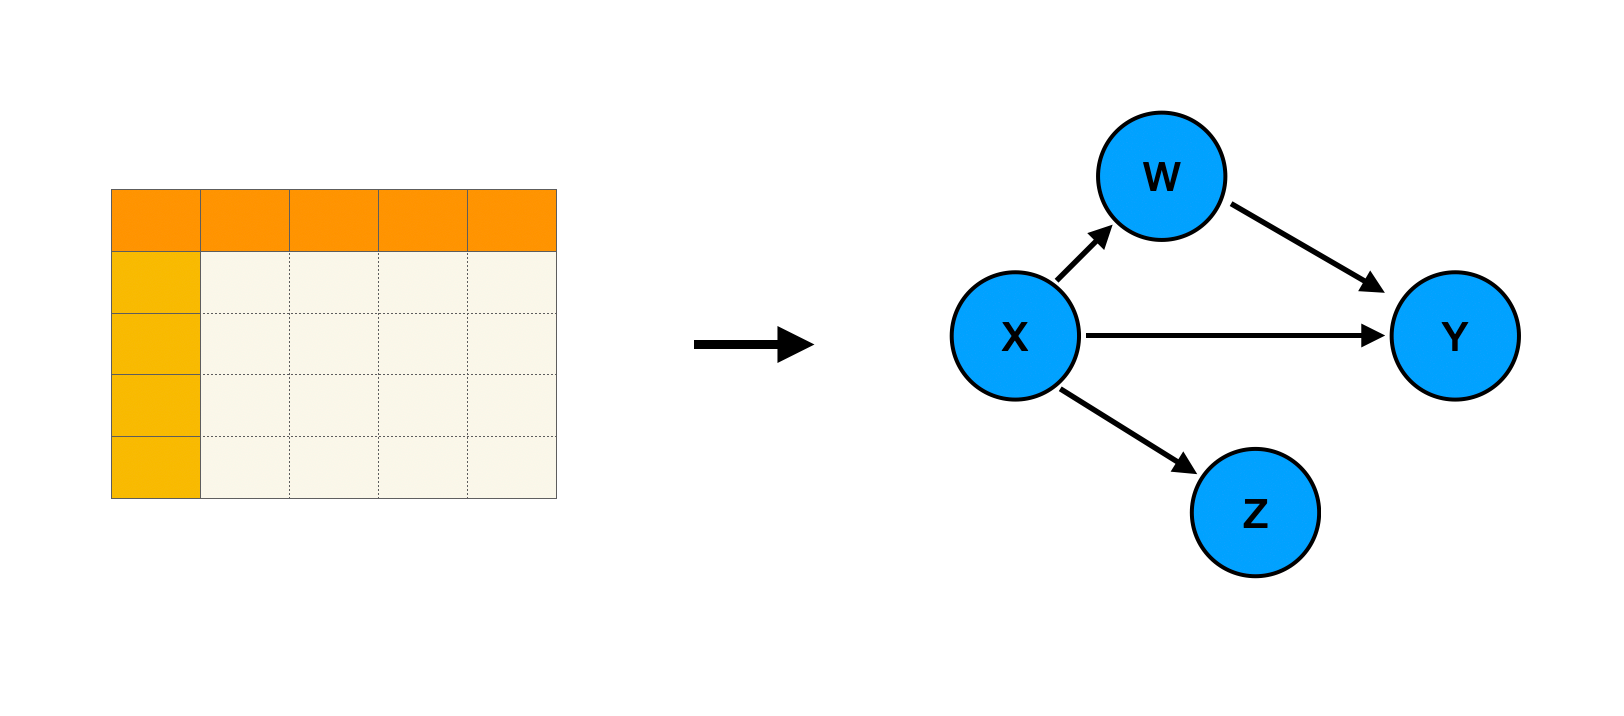
\includegraphics[width=0.75\textwidth]{figures/causal_discovery.png}
    \end{figure}
\end{frame}

\begin{frame}{Descoberta Causal}
    Dados observacionais sozinhos geralmente identifica apenas a classe de equivalência representado por um \textit{CPDAG} (Completed Partially Directed Acyclic Graph) e não um único DAG.

    \pause

    O problema é muito desafiador por diversos motivos:
    \begin{itemize}
        \item O espaço de busca de possíveis grafos cresce super-exponencialmente com o número de variáveis;
        \pause
        \item Amostras finitas podem fornecer estimativas não confiáveis de independências condicionais;
        \pause
        \item A presença de variáveis latentes (não observadas) pode impedir que a verdadeira estrutura seja identificada apenas com dados.
    \end{itemize}
\end{frame}

\begin{frame}{Descoberta Causal}{Famílias de abordagens}
    \begin{itemize}
        \item \textbf{Constraint-based}: Utiliza testes de independência condicional para inferir a estrutura causal. Exemplo: PC, FCI.
        \pause
        \item \textbf{Score-based}: Busca por uma estrutura que maximize uma função de pontuação (score) equilibrando fit e complexidade. Exemplo: GES, BIC.
        \pause
        \item \textbf{Functional}: Explora assimetrias na forma funcional de relações entre variáveis para inferir causalidade. Exemplo: LiNGAM, ANM. - Assumem relações lineares e sem ruído gaussiano, podendo identificar até um DAG completo, se as premissas forem atendidas.
        \pause
        \item \textbf{Hybrid}: Combina elementos de diferentes abordagens.
    \end{itemize}
\end{frame}

\begin{frame}{Descoberta Causal}{Escolhendo um algoritmo de CD}
    \begin{columns}[T]
        \begin{column}{0.25\textwidth}
            \begin{figure}
                \centering
                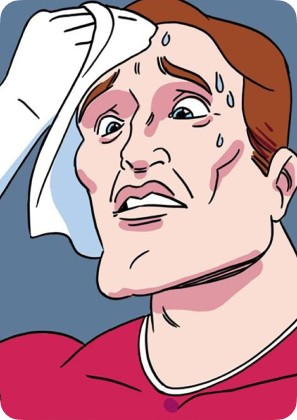
\includegraphics[width=0.9\textwidth]{figures/choice_guy.jpg}
            \end{figure}
        \end{column}
        \begin{column}{0.75\textwidth}
            Escolher um algoritmo de CD depende de características como:
            \begin{itemize}
                \item Tamanho do conjunto de dados (número de amostras e variáveis);
                \pause
                \item Premissas sobre a distribuição dos dados (linearidade, ruído, etc.);
                \pause
                \item Tipos de dados suportados (contínuos, discretos);
                \pause
                \item Robustez a ruído e outliers.
            \end{itemize}
            \pause
            Não existe bala de prata. \\ Na prática, é comum testar vários e buscar um consenso ou utilizar conhecimento de negócio para validar os resultados.
        \end{column}
    \end{columns}
\end{frame}

\begin{frame}[plain]
    \begin{table}[htbp]
    \centering
    \label{tab:discovery_algorithms}
    \footnotesize
    \begin{tabular}{llccc}
    \toprule
    \textbf{Algorithm} & \textbf{Full Name} & \makecell{\textbf{Supported} \\ \textbf{Data Types}} & \makecell{\textbf{Gaussian} \\ \textbf{Assumption}} & \textbf{Family} \\
    \midrule
    PC \cite{discovery-pc} & Peter-Clark & C, D & No & Constraint \\
    GS \cite{discovery-gs} & Grow-Shrink & C, D & No & Constraint \\
    IAMB \cite{discovery-iamb} & Incremental Assoc. Markov Blanket & C, D & No & Constraint \\
    Fast-IAMB \cite{discovery-iamb-variants} & Fast Markov Blanket & C, D & No & Constraint \\
    Inter-IAMB \cite{discovery-iamb-variants} & Interleaved Markov Blanket & C, D & No & Constraint \\
    MMPC \cite{discovery-mmpc} & Max-Min Parents and Children & C, D & No & Constraint \\
    \midrule
    GES \cite{discovery-ges} & Greedy Equivalence Search & C, D & Yes & Score \\
    GIES \cite{discovery-ges_gies} & Greedy Interv. Equivalence Search & C, D & Yes & Score \\
    CCDr \cite{discovery-ccdr} & Concave penalized Coord. Descent & C & Yes & Score \\
    BES \cite{discovery-bes} & Bayesian Equivalence Search & C, D & Yes & Score \\
    CGNN \cite{discovery-cgnn} & Causal Generative Neural Networks & C & No & Score \\
    SAM \cite{discovery-sam} & Structural Agnostic Model & C & No & Score \\
    \midrule
    LiNGAM \cite{discovery-lingam} & Linear Non-Gaussian Acyclic Model & C & No\textsuperscript{*} & Functional \\
    CAM \cite{discovery-cam} & Causal Additive Models & C & Yes & Functional \\
    \midrule
    GRaSP \cite{discovery-grasp} & Greedy Relax. of Sparsest Perm. & C, D & No & Hybrid \\
    \bottomrule
    \multicolumn{5}{l}{\scriptsize \textsuperscript{*}LiNGAM assumes linear relationships with non-Gaussian noise.}
    \end{tabular}
    \end{table}
\end{frame}

\begin{frame}{Mão na massa}
	\notebooklink{2}{2\_causal\_discovery.ipynb}
\end{frame}

\section{Inferência Causal}

\begin{frame}{Inferência Causal}
    Causal Discovery (CD) aprende a estrutura de relações causais. Causal Inference (CI) estima a magnitude dos efeitos causais.

    \vfill

    CI responde perguntas como ''Qual é o efeito do tratamento \bm{$X$} no resultado \bm{$Y$}?''.

    \begin{figure}
        \centering
	    
\includegraphics[width=0.75\linewidth]{figures/homer_potential_outcomes.jpg}
    \end{figure}
\end{frame}

\begin{frame}{Inferência Causal}{Identificação}
    Antes de calcular qualquer coisa, precisamos responder uma pergunta mais básica: \textbf{dá pra calcular esse efeito com os dados que eu tenho?}

    \pause

    Um efeito é \textit{identificável} se puder ser determinado unicamente a partir dos dados observacionais e do grafo causal. Se o grafo tiver um confundidor que você não mediu, por exemplo, a resposta pode ser \textbf{não}. Não importa o quão sofisticado seja o seu método depois.

    \pause

    \vfill
    Na prática, quem responde essa pergunta é o \textit{do-calculus} de Pearl: um conjunto de regras formais para isso. Não vamos entrar nas regras; o que importa é a ideia: \textbf{identificação vem antes de estimação}.
\end{frame}

\begin{frame}{Inferência Causal}{O que esse número quer dizer?}
    Lembra do efeito individual \bm{$\tau_i = Y_i(1) - Y_i(0)$} da seção anterior? O \textbf{ATE} (Average Treatment Effect) é só a média disso para todo mundo:

    \vspace{10pt}
    \centering \bm{$\tau = \text{média de } \tau_i \text{ na população}$}
    \raggedright

    \vspace{15pt}
    \pause

    Isso é um número que você pode interpretar direto, como uma métrica de negócio. Ex: efeito de um programa de treinamento profissional no salário anual.

    \pause
    \begin{itemize}
        \item \bm{$\tau = \$20.000$} \pause $\to$ o programa muda a vida da pessoa;
        \item \bm{$\tau = \$1.794$} \pause $\to$ efeito modesto, só algumas semanas de salário a mais por ano;
        \item \bm{$\tau = \$2$} \pause $\to$ estatisticamente é ruído, não é um efeito de verdade;
        \item \bm{$\tau = -\$500$} \pause $\to$ o programa parece estar \textit{piorando} a vida das pessoas.
    \end{itemize}
\end{frame}

\begin{frame}{Inferência Causal}{Por que não posso só comparar as médias?}
    Resposta curta: \textbf{confundimento} (aquele fork que vimos antes: \bm{$X \leftarrow Z \rightarrow Y$}).

    \pause
    \vfill

    Suponha os dados:
    \begin{itemize}
        \item Média(salário $\mid$ fez o programa) $-$ Média(salário $\mid$ não fez) \bm{$= -\$8.497$} \pause \alert{(!)}
        \item Efeito causal real, medido em um experimento controlado: \bm{$\tau = \$1.794$}
    \end{itemize}

    \pause
    \vfill
    A comparação direta não só erra o valor, ela erra o \textbf{sinal}. Quem fez o programa, na média, já ganhava menos antes de entrar nele;
    
    Comparar as médias brutas confunde ''efeito do programa'' com ''quem tende a se inscrever no programa''.
\end{frame}

\begin{frame}{Inferência Causal}{Como os métodos corrigem isso?}
    A ideia por trás de (quase) todo estimador é a mesma: \textbf{comparar pessoas parecidas entre si}, e só depois olhar a diferença de tratamento. Não vamos ver as fórmulas, só a lógica de cada um:

    \pause
    \begin{itemize}
        \item \textbf{Ajuste por regressão}: aprende um modelo do resultado e usa ele pra simular ''e se essa pessoa tivesse (ou não) feito o tratamento?'';
        \pause
        \item \textbf{Pareamento (\textit{matching})}: pra cada pessoa tratada, acha um ''gêmeo estatístico'' não tratado (o mais parecido possível) e compara os dois;
        \pause
        \item \textbf{Score de propensão / IPW}: dá mais peso a quem é ''raro'' no seu grupo, pra reequilibrar a comparação;
        \pause
        \item \textbf{Estimadores duplamente robustos}: usa duas das ideias acima ao mesmo tempo, como uma rede de segurança: se uma errar, a outra ainda salva a estimativa.
    \end{itemize}
\end{frame}

\begin{frame}{Inferência Causal}{O valor bruto é comparável entre datasets?}
    Em ML, temos dois tipos de métrica:
    \begin{itemize}
        \item \textbf{Padronizadas}: acurácia, AUC, F1, R²... vivem numa escala fixa e dá pra comparar entre problemas diferentes, mais ou menos;
        \pause
        \item \textbf{Na escala bruta}: RMSE, MAE... um RMSE de 5 não quer dizer nada sozinho, depende da unidade do que você está prevendo.
    \end{itemize}

    \pause
    \textbf{O efeito causal (\bm{$\tau$}) é sempre do segundo tipo.} Ele vive na escala original do resultado \bm{$Y$}. Não existe uma versão ``padronizada e universal'' por padrão.

    \pause
    \begin{itemize}
        \item \bm{$\tau = 1.794$} em dólares de salário $\neq$ \bm{$\tau = 1.794$} em mmHg de pressão $\neq$ \bm{$\tau = 1.794$} em cliques de anúncio;
        \pause
        \item O mesmo número pode ser \textbf{enorme} num contexto e \textbf{irrelevante} em outro.
    \end{itemize}

    \pause
    \bm{$\tau_{\text{Grafo A}}$} $>$ \bm{$\tau_{\text{Grafo B}}$} \textbf{não} necessariamente significa ``o efeito em A é maior''.
\end{frame}

\begin{frame}{Inferência Causal}{Como confiar no número?}
    Diferente de um modelo preditivo, aqui não existe um ''conjunto de teste'' óbvio pra validar a resposta.
    
    Afinal, nós nunca observamos o contrafactual.
    
    Então, em vez de provar que a estimativa está certa, tentamos \textbf{quebrar ela} de propósito.

    \begin{figure}
        \centering
        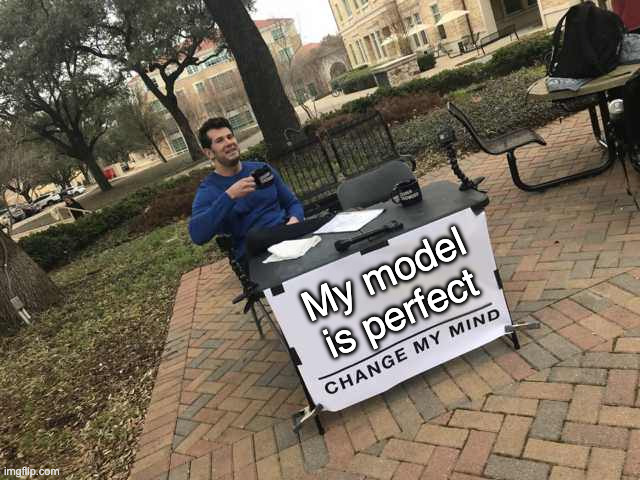
\includegraphics[width=0.45\linewidth]{figures/meme-changemymind.jpg}
    \end{figure}
\end{frame}
\begin{frame}{Inferência Causal}{Como confiar no número?}
    \begin{itemize}
        \item \textbf{Teste placebo}: aplique o mesmo método em algo que você \textit{sabe} que não tem efeito nenhum (ex: um tratamento sorteado aleatoriamente). Se o método ''encontra'' um efeito mesmo assim, desconfie dele;
        \pause
        \item \textbf{Subconjuntos de dados}: repita a análise em pedaços diferentes dos dados. Se o número fica pulando de um lado pro outro, sua estimativa não é tão sólida quanto parece;
        \pause
        \item \textbf{Causa comum aleatória}: adicione uma variável de ruído qualquer, como se fosse um confundidor. Um bom método deve ignorar ela e manter a estimativa praticamente igual.
    \end{itemize}

    \pause
    Nenhum desses testes \textit{prova} que a estimativa está certa,só avaliam sua confiança nela.
\end{frame}

\begin{frame}{Inferência Causal}{Juntando Tudo}
    \begin{figure}
        \centering
        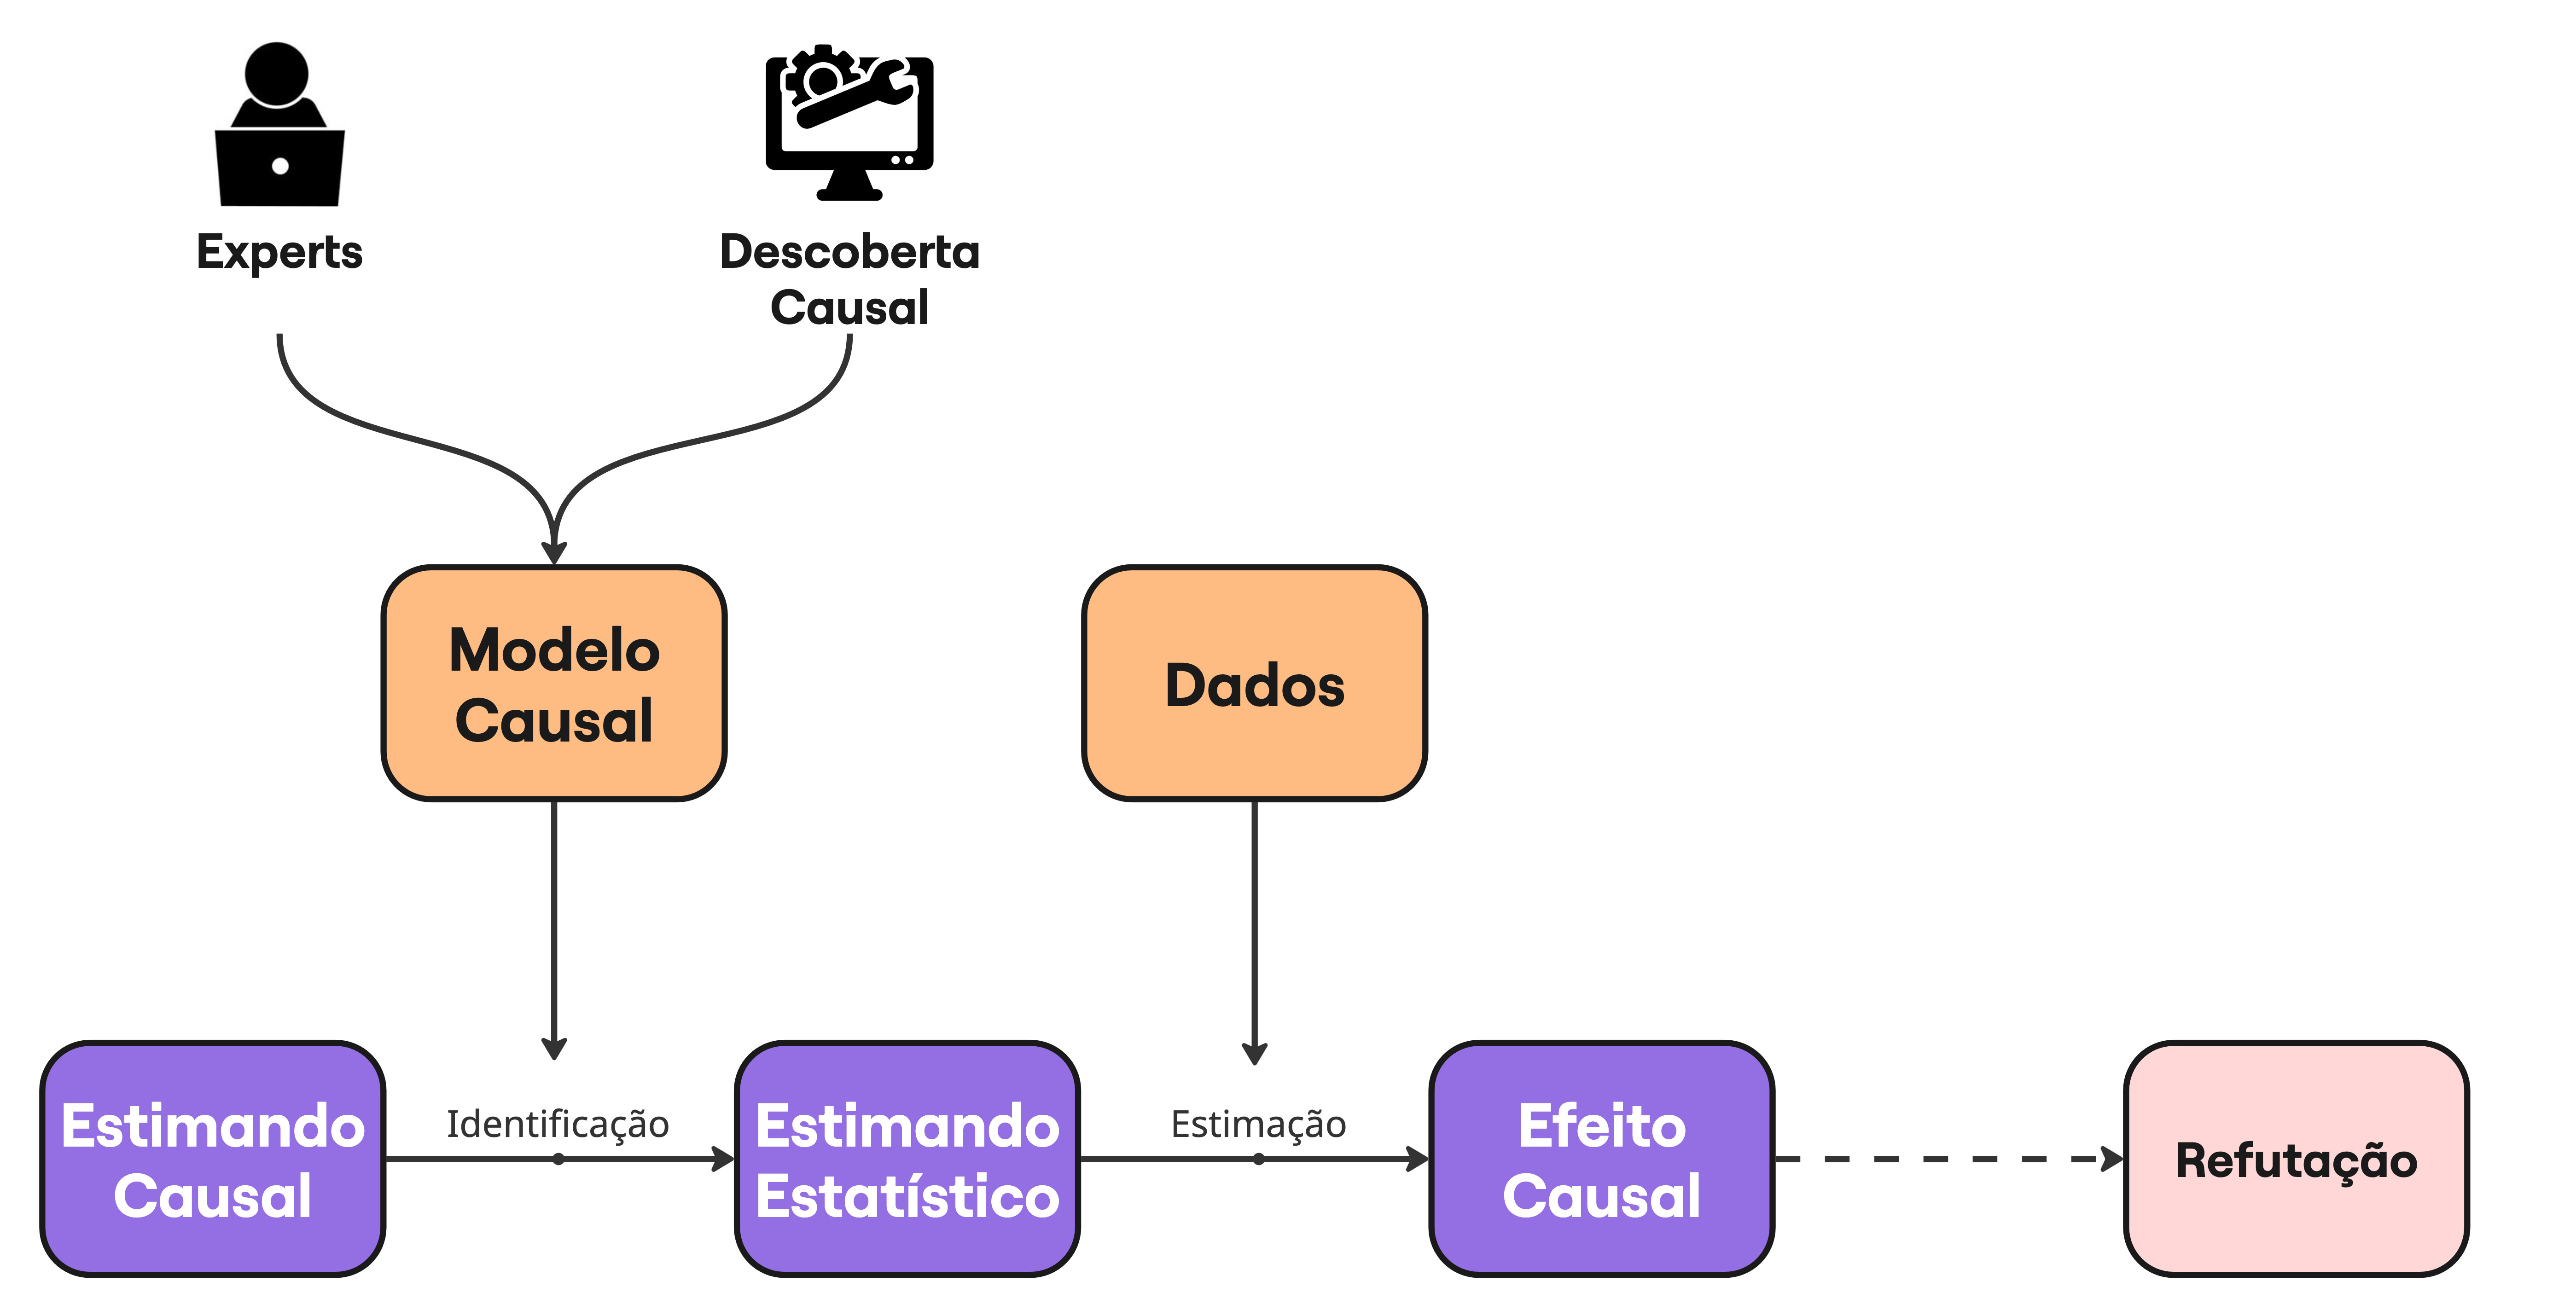
\includegraphics[width=1.0\framewidth]{figures/causal_inference_flow.jpg}
    \end{figure}
\end{frame}


\begin{frame}{Mão na massa}
	\notebooklink{3}{3\_causal\_estimation.ipynb}
\end{frame}

\begin{frame}[plain]{Inferência Causal}{E se o efeito não for igual pra todo mundo?}
    O ATE é uma média sobre toda a população. Só que médias escondem coisa.

    \pause
    Imagine um tratamento que ajuda metade das pessoas e atrapalha a outra metade, na mesma proporção. \pause O ATE dá quase zero \pause mas não porque o tratamento não faz nada, e sim porque os efeitos opostos se cancelam.

    \pause
    \vfill
    \begin{center}
        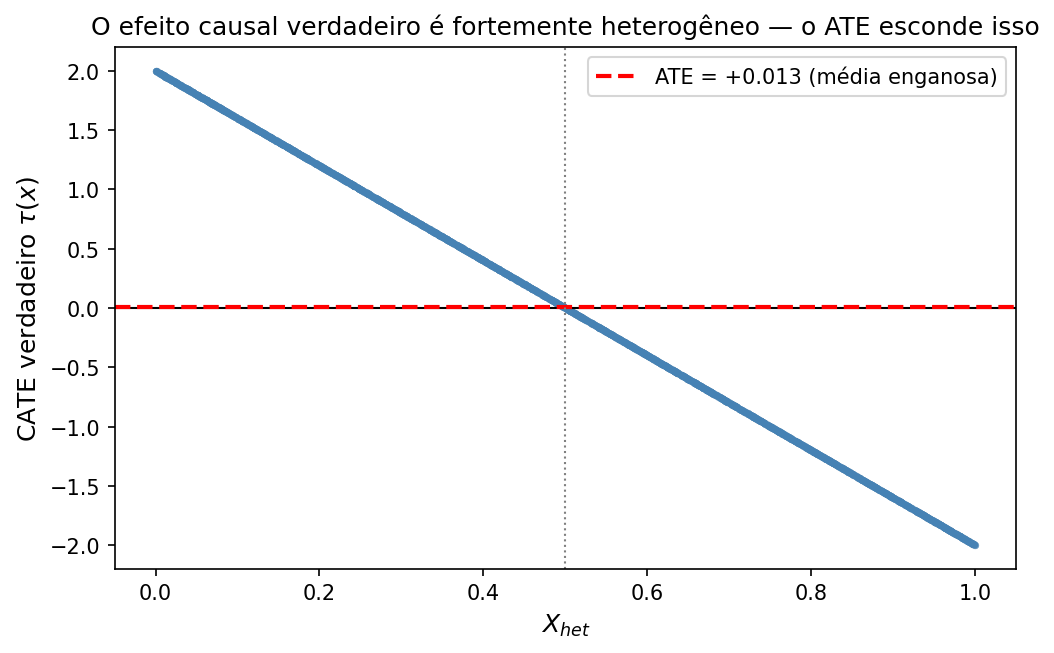
\includegraphics[width=0.625\linewidth]{figures/5_true_cate.png}
    \end{center}
\end{frame}

\begin{frame}{Inferência Causal}{CATE: o mesmo efeito, agora por subgrupo}
    O \textbf{CATE} (\textit{Conditional Average Treatment Effect}) responde: qual o efeito do tratamento, condicionado nas covariáveis \bm{$X$}?

    \vspace{10pt}
    \centering \bm{$\tau(x) = \mathbb{E}[Y(1) - Y(0) \mid X = x]$}
    \raggedright

    \pause
    \vspace{15pt}
    É a mesma ideia do ATE que você já viu, só que calculada separadamente pra cada perfil de unidade, em vez de uma média só pra todo mundo.

    \pause
    \vfill
    Com isso dá pra tomar uma decisão \textbf{personalizada}: trate a unidade \bm{$i$} só se \bm{$\hat\tau(x_i) > 0$}. Situações assim são comuns em saúde (um remédio ajuda um genótipo e prejudica outro) e marketing (uma promoção atrai quem é sensível a preço e irrita quem já é cliente fiel).
\end{frame}

\begin{frame}{Inferência Causal}{Meta-learners: estimando o CATE}
    A ideia por trás dos métodos mais comuns (\textit{meta-learners}) reaproveita os mesmos estimadores de ATE que você já viu, só que combinados de um jeito diferente:
    \begin{itemize}
        \item \textbf{S-learner}: um modelo só, com o tratamento como mais uma variável;
        \pause
        \item \textbf{T-learner}: dois modelos separados, um pra cada braço do tratamento;
        \pause
        \item \textbf{X-learner}: usa os dois modelos do T-learner pra imputar o efeito individual, útil quando os grupos são desbalanceados.
    \end{itemize}

    \begin{alertblock}{Notebook extra!}
		Caso queira aprofundar nesse assunto, veja o notebook extra \#5.
	\end{alertblock}
\end{frame}

\section{Ferramentas e Datasets}

\begin{frame}{Ferramentas e Datasets}
    Você já viu o pipeline inteiro: descoberta, identificação, estimação, refutação.

    \pause
    \vfill
    Pergunta que todo mundo faz depois de um curso de causalidade: \textbf{``beleza, mas eu clico em quê pra fazer isso?''}

    \begin{figure}
        \centering
        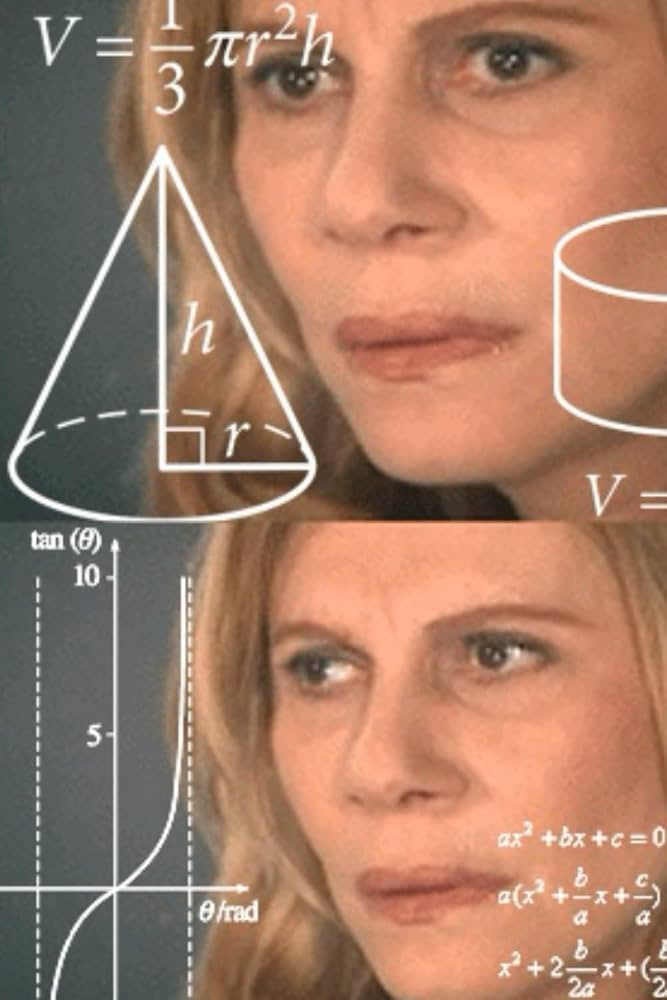
\includegraphics[width=0.2\linewidth]{figures/nazare.jpg}
    \end{figure}
\end{frame}

\begin{frame}[plain]
    \begin{table}[htbp]
    \centering
    \label{tab:causal_tools}
    \small
    \begin{tabular}{lccccc}
    \toprule
    \textbf{Ferramenta} & \textbf{Descoberta} & \textbf{Estimação} & \textbf{Refutação} & \textbf{Interface} & \textbf{Paralelo} \\
    \midrule
    CDT \cite{tool-causaldiscoverytoolbox} & \checkmark & -- & -- & -- & -- \\
    causal-learn \cite{tool-causallearn} & \checkmark & -- & -- & -- & -- \\
    bnlearn \cite{tool-bnlearn} & \checkmark & -- & -- & -- & -- \\
    Tetrad \cite{tool-tetrad} & \checkmark & -- & -- & \checkmark & -- \\
    gCastle \cite{tool-gcastle} & \checkmark & -- & -- & -- & -- \\
    DoWhy \cite{ai-sharma2020dowhy} & -- & \checkmark & \checkmark & -- & -- \\
    EconML \cite{tool-econml} & -- & \checkmark & -- & -- & -- \\
    CausalML \cite{ai-chen2020causalml} & -- & \checkmark & -- & -- & \checkmark \\
    CausalNex \cite{tool-causalnex} & \checkmark & \checkmark & -- & -- & -- \\
    Salesforce CausalAI \cite{tool-salesforce-causalai} & \checkmark & -- & -- & \checkmark & \checkmark \\
    \textit{Causal-Nest} \cite{causal-nest-kbs} & \checkmark & \checkmark & \checkmark & -- & \checkmark \\
    \bottomrule
    \end{tabular}
    \end{table}
\end{frame}

\begin{frame}{Ferramentas}{Um problema meio óbvio}
    Repara no padrão da tabela: \pause praticamente ninguém faz tudo.

    \pause
    \begin{itemize}
        \item Ferramentas de \textbf{descoberta} (CDT, causal-learn, bnlearn, Tetrad, gCastle) sabem achar a estrutura, mas não estimam nem refutam nada;
        \pause
        \item Ferramentas de \textbf{inferência} (DoWhy, EconML, CausalML) já assumem que você chegou com um grafo pronto na mão.
        \item Alguns backends em R; as representações de grafo são diferentes, etc.
    \end{itemize}

    \pause
    \vfill
    Na prática, isso significa juntar ferramentas diferentes manualmente: converter formato de dado, e torcer pra estrutura descoberta bater com o que a ferramenta de inferência espera.

    \pause
    \vfill
    O \textit{Causal-Nest} (projeto do autor) é uma tentativa de unificar esse pipeline inteiro numa única interface.
\end{frame}

\begin{frame}{Datasets}{Onde está o gabarito?}
    Em ML supervisionado, você tem o rótulo verdadeiro pra comparar. Em CD, isso quase nunca acontece: o grafo causal ``de verdade'' por trás de um dataset observacional raramente é conhecido com certeza.

    \pause
    \vfill
    O \textbf{Sachs}, que a gente usou lá no Notebook 2, é a exceção rara: um dos poucos datasets reais com grafo verdadeiro validado por experimentos de intervenção de verdade.

    \pause
    \vfill
    A grande maioria dos outros benchmarks conhecidos não tem um grafo completo. Eles trazem, no máximo, pistas parciais: ordem temporal entre variáveis, ou uma lista de arestas proibidas e obrigatórias.
\end{frame}

\begin{frame}{O ``Expert'' no meio do pipeline?}
    Lembra dessa figura?

    \begin{figure}
        \centering
        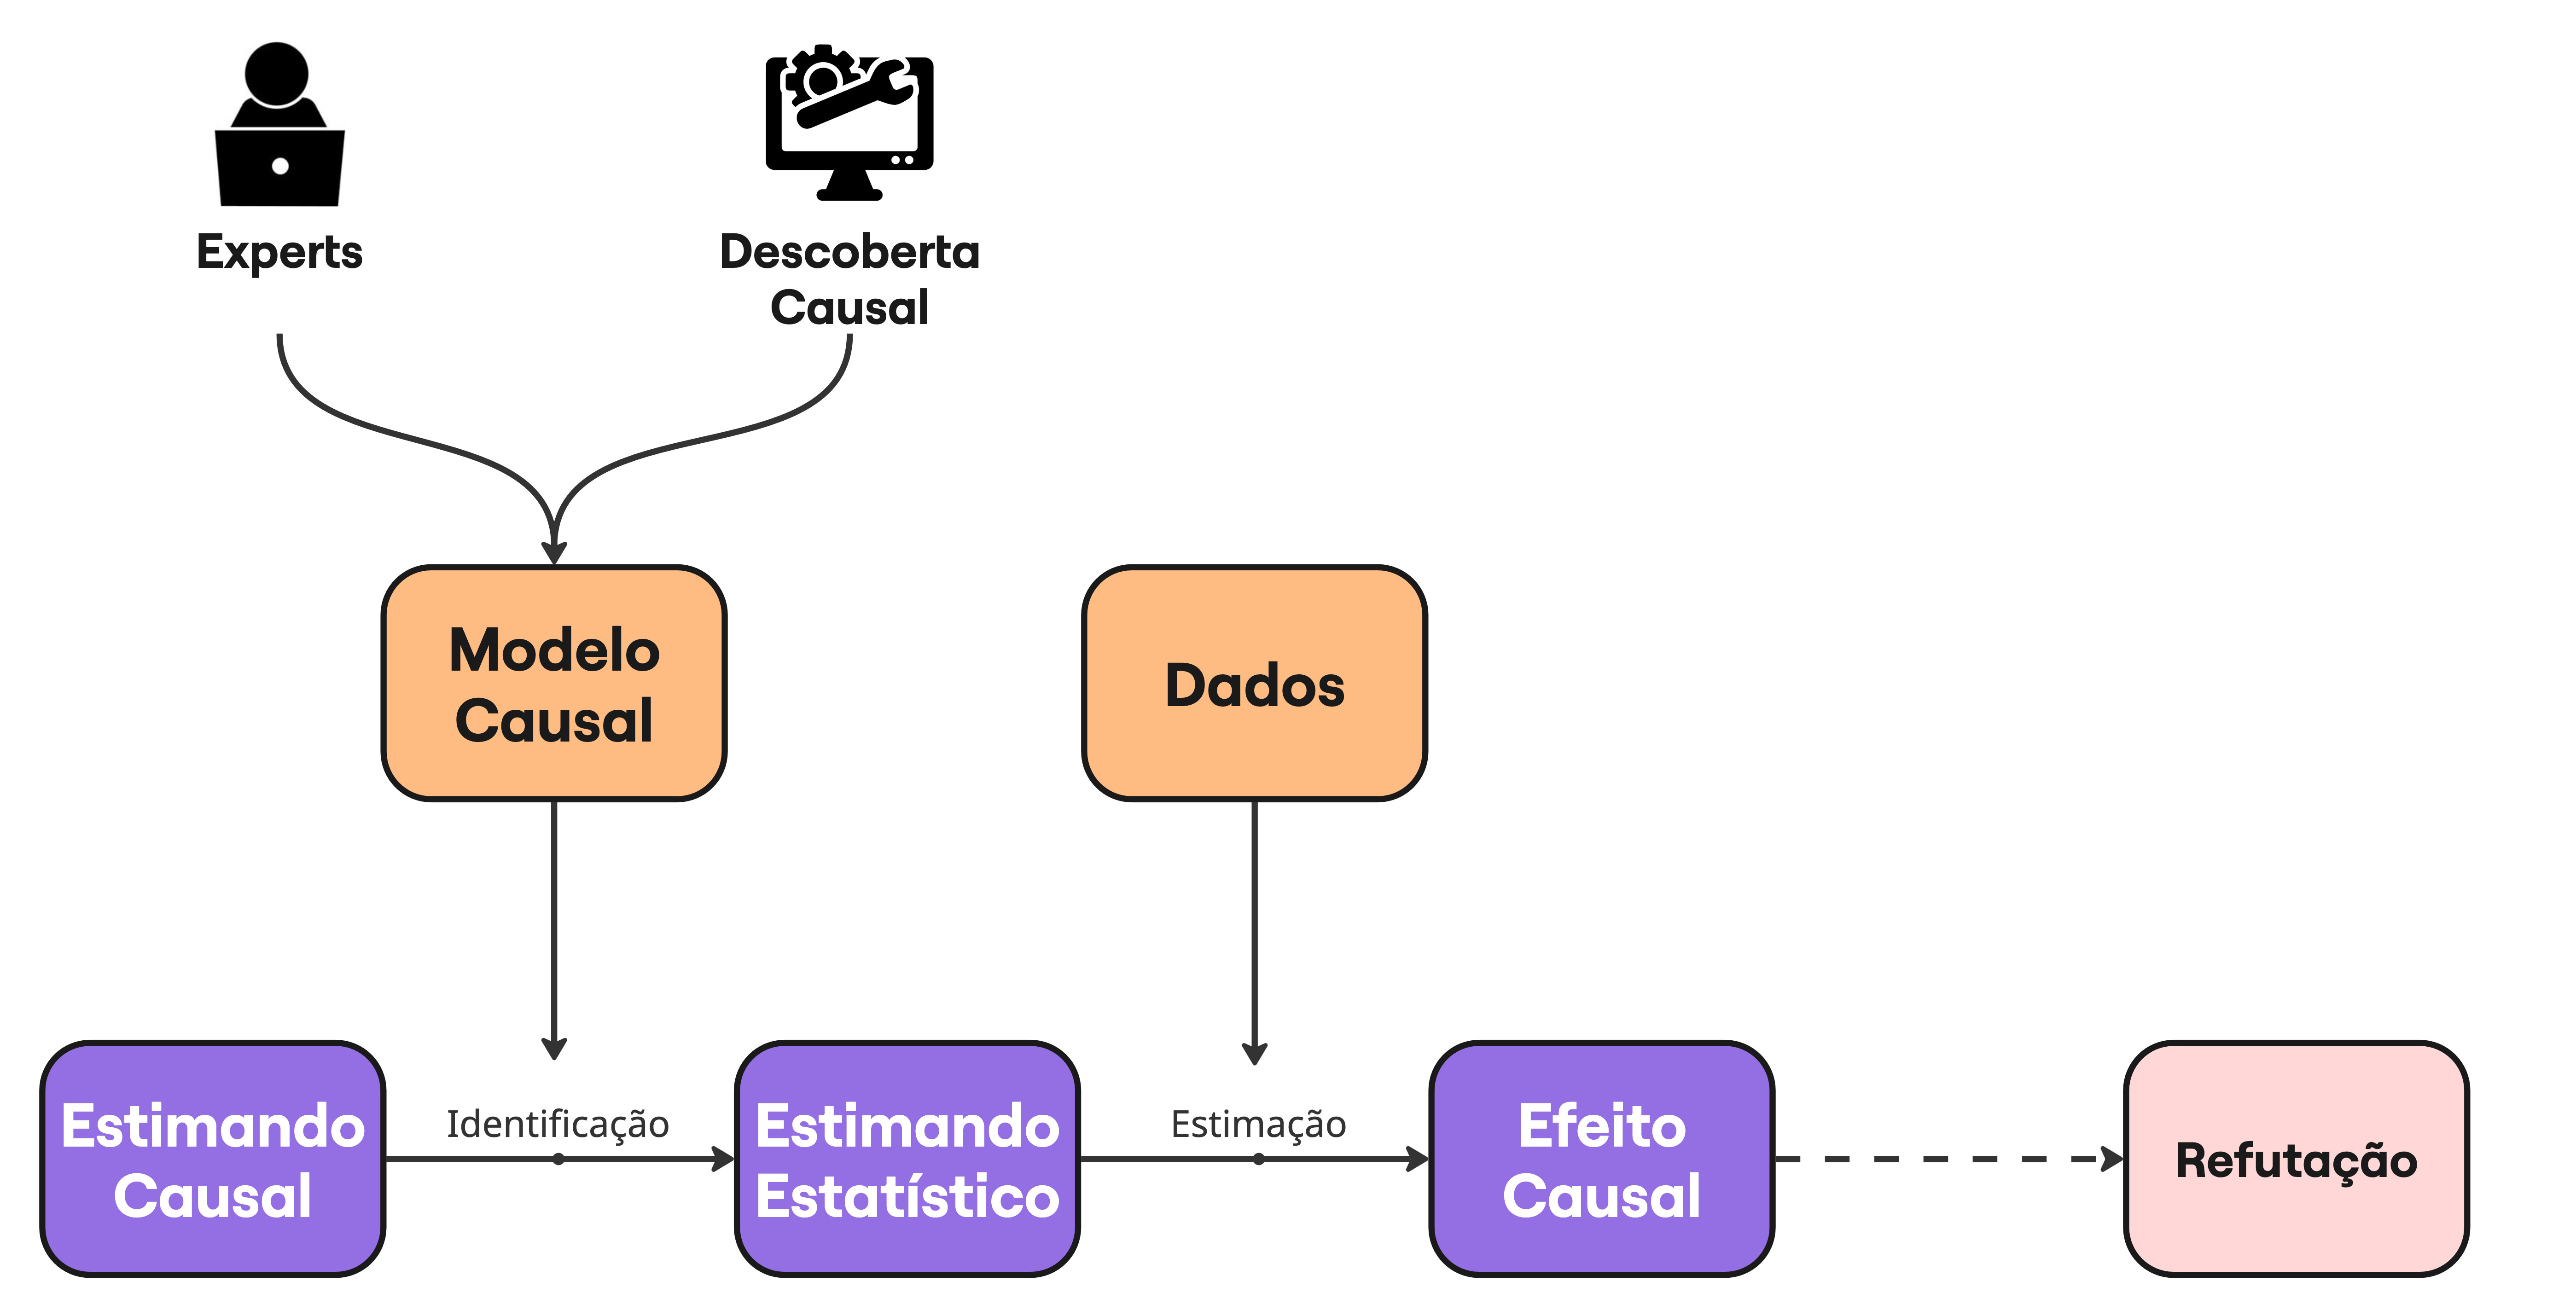
\includegraphics[width=0.5\textwidth]{figures/causal_inference_flow.jpg}
    \end{figure}

    \pause
    Sem dataset de gabarito pra validar automaticamente, alguém precisa olhar o grafo e dizer ``faz sentido'' ou ``essa seta tá errada''.
    
    \pause
    Na prática, CD quase sempre entrega uma sugestão, não uma resposta final. Um humano com conhecimento de domínio é necessário pra ter uma resposta causal válida de fato.
\end{frame}

\begin{frame}{Quer dizer que é inútil sem um especialista?}
    \begin{figure}
        \centering
        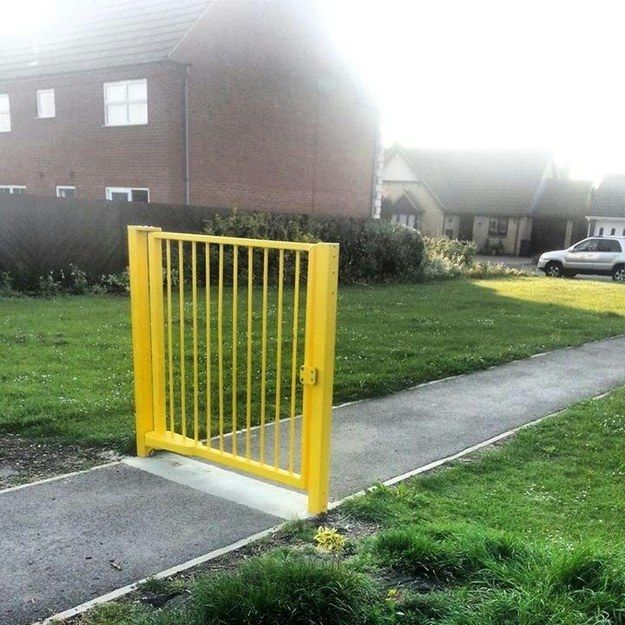
\includegraphics[width=0.22\textwidth]{figures/useless.jpg}
    \end{figure}

    \pause
    \texttt{\Large{NÃO!}}

    Mesmo sem um especialista, a análise automatizada de causalidade pode ser útil para melhorar a compreensão do problema, gerar hipóteses, e até mesmo melhorar modelos preditivos.

    \pause

    Afinal, modelos baseados apenas em correlação não são úteis?
\end{frame}

\begin{frame}{Mão na massa}
	\notebooklink{4}{4\_causal\_feature\_selection.ipynb}
\end{frame}
\section{Explicabilidade Causal}

\begin{frame}{Explicabilidade Causal}{De volta à Hierarquia de Pearl}
    Lembra da Hierarquia Causal? \pause O nível 3, \textit{counterfactual}, pergunta ``e se eu tivesse agido diferente?''. 

    É exatamente a pergunta que aparece quando alguém quer entender (ou contestar) uma decisão automatizada.

    \pause
    \vfill
    Duas famílias de explicação, duas perguntas bem diferentes:
    \begin{itemize}
        \item \textbf{SHAP} (atribuição): ``o que pesou nessa previsão?'';
        \pause
        \item \textbf{DiCE} (contrafactual): ``o que eu precisaria mudar pra mudar o resultado?''.
    \end{itemize}
\end{frame}

\begin{frame}{Explicabilidade Causal}{SHAP vs. Contrafactual, num exemplo real}
    \begin{columns}[T]
        \begin{column}{0.52\textwidth}
            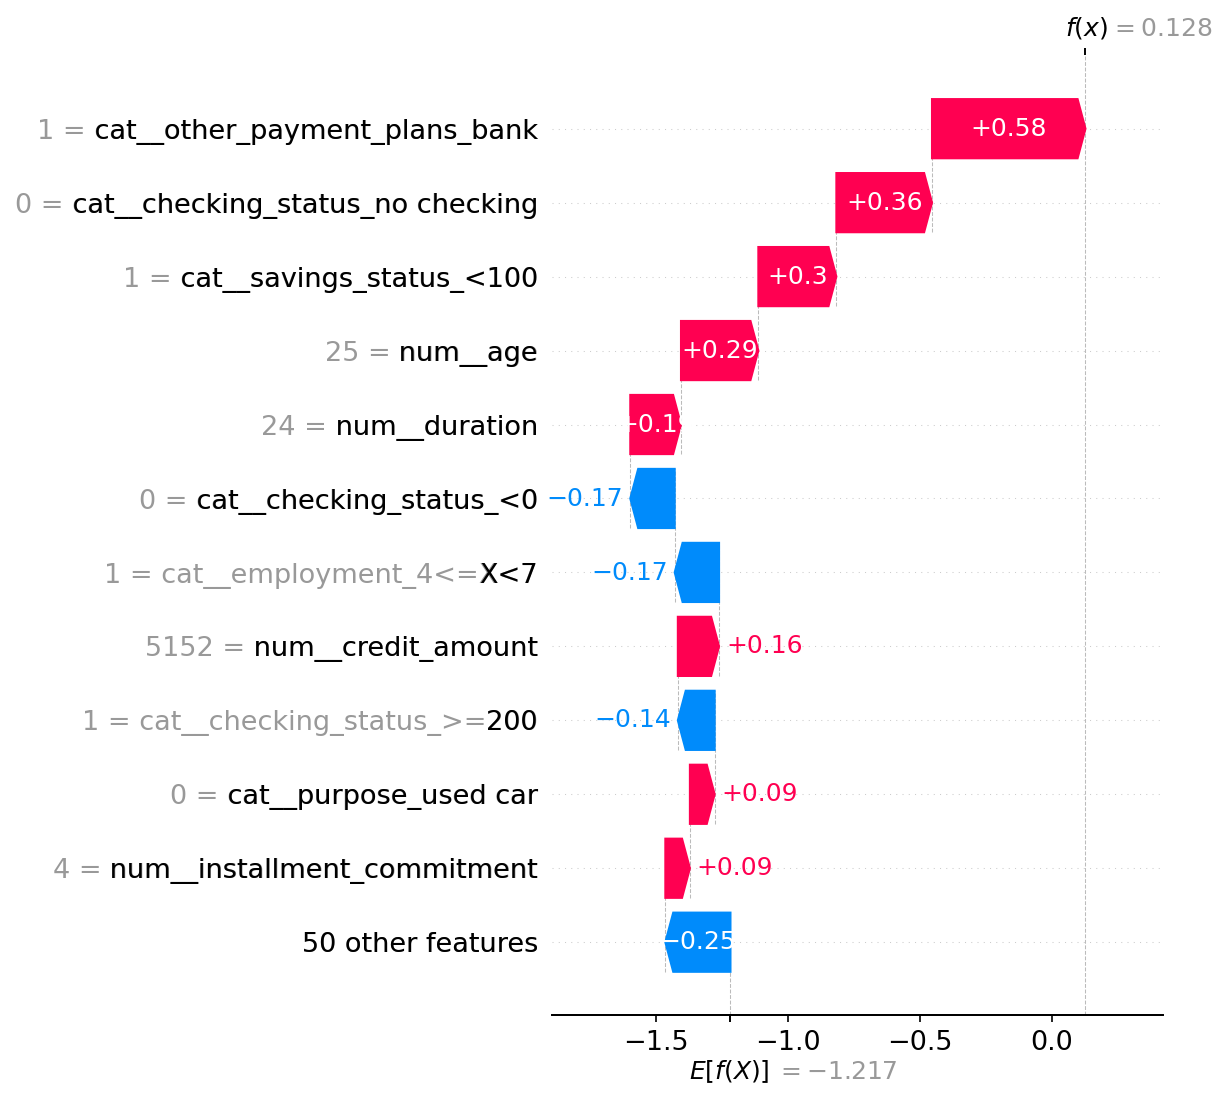
\includegraphics[width=\linewidth]{figures/7_shap_waterfall.png}
        \end{column}
        \begin{column}{0.48\textwidth}
            Esse é um SHAP \textit{waterfall} de um pedido de crédito negado.

            \vspace{10pt}
            Ele diz o que ``pesou'' na decisão do modelo... \pause mas não diz o que fazer a respeito.

            \pause
            \vspace{10pt}
            E se um dos atributos que mais pesou for algo que a pessoa não pode simplesmente mudar (idade, nacionalidade)?
        \end{column}
    \end{columns}
\end{frame}

\begin{frame}{Explicabilidade Causal}{Contrafactuais precisam de causalidade}
    Um gerador de contrafactuais sem nenhuma restrição pode sugerir ``mude sua idade de 25 pra 65'', o que é matematicamente válido, mas impossível na vida real.

    \pause
    \vfill
    A correção natural é usar o grafo causal: restringir a busca só a atributos \textit{mutáveis}, e propagar mudanças pelos seus efeitos causais (ex: aumentar o tempo de emprego também deveria mudar a renda esperada).

    \pause
    \vfill
    É a mesma lição do curso inteiro, aplicada em outro lugar: \textbf{o grafo carrega as suas suposições}, e ignorá-lo tem custo prático, não só teórico.

    \begin{alertblock}{Notebook extra!}
		Caso queira aprofundar nesse assunto, veja o notebook extra \#6.
	\end{alertblock}
\end{frame}

% Conclusão, referências --------------------------------------------------
\section{Conclusão}

\begin{frame}{Aprendizados}
	\begin{itemize}
		\item \textbf{Correlação $\neq$ causalidade}: o Paradoxo de Simpson mostrou isso com dados reais de vacinação, agregando errado, a vacina parecia piorar as coisas;
		\pause
		\item Um \textbf{grafo causal} formaliza suas suposições. Ele vem de especialistas, de descoberta automática, ou (o mais realista) dos dois juntos;
		\pause
		\item \textbf{Causal Discovery} entrega uma classe de equivalência, não necessariamente a verdade.
		\pause
		\item \textbf{Identificar $\to$ Estimar $\to$ Refutar} é um pipeline, não uma fórmula única.
		\pause
		\item Causalidade \textbf{não exige um especialista o tempo todo}. Ex: seleção causal de atributos sem ninguém desenhando grafo à mão foi a diferença entre um modelo que quebra sob intervenção e um que não quebra.
	\end{itemize}
\end{frame}

\begin{frame}{Desafios Abertos}
	Agora que você conhece um pouco mais sobre causalidade, talvez tenha percebido que ainda existem alguns desafios abertos:

	\begin{itemize}
		\item \textbf{Curva de aprendizado íngreme}: vocabulário, suposições e formalismo matemático são bem diferentes do que se vê em áreas como ML tradicional;
		\pause
		\item \textbf{Ferramentas fragmentadas}: você viu a tabela, quase ninguém faz descoberta, estimação e refutação ao mesmo tempo;
		\pause
		\item \textbf{Escolher o algoritmo de descoberta certo é confuso}: PC? GES? LiNGAM? A resposta depende de premissas que muitas vezes você nem sabe se valem pro seu dataset;
		\pause
		\item \textbf{As ferramentas não conversam entre si}: montar um pipeline automatizado de ponta a ponta hoje é, na prática, trabalho manual de encaixar peças.
	\end{itemize}
\end{frame}

\begin{frame}{Sobre o Causal-Nest}
	Foi exatamente pra atacar esses quatro problemas que desenvolvemos o \textbf{Causal-Nest} \cite{causal-nest-kbs}: um framework que junta descoberta, validação de grafo, estimação e refutação num só pipeline, com interface web pra reduzir a barreira de entrada pra quem não é especialista.

	\pause
	\vfill
	Não vamos entrar em detalhes aqui (é assunto pra outro curso!), mas se você curtiu a ideia e quiser se aprofundar:

	\begin{center}
		\textbf{Causal-Nest: A framework for automated causal discovery and inference} 
		\small \href{https://doi.org/10.1016/j.knosys.2026.116005}{doi.org/10.1016/j.knosys.2026.116005} \\
		\textit{Knowledge-Based Systems}, v.~343 (2026)
	\end{center}
\end{frame}

\begin{frame}{De onde vem esse curso}
	Boa parte do conteúdo teórico apresentado aqui foi originalmente escrito como o capítulo teórico da minha dissertação de mestrado na UFV \cite{diss-viegas2026}, sob orientação de Fabrício Aguiar Silva e Marcus Henrique Soares Mendes.

	\pause
	\vfill
	Se você quiser ver a mesma ideia de engenharia causal de atributos aplicada com mais profundidade num problema real, temos um estudo publicado no CBIC 2025 \cite{CBIC2025-1175578}: usamos o Causal-Nest pra guiar a engenharia de atributos na previsão de churn de clientes de telecom, e o ganho apareceu de forma consistente em vários modelos de ML diferentes.
\end{frame}

\begin{frame}{Materiais Extras}
	\begin{itemize}
		\item \textbf{Vídeo/slides complementares} \\
		\href{https://drive.google.com/file/d/1ghmXMiwcGzTnbcT2gYuuKWE01T1wBTdJ/view?usp=sharing}{Causal Representation Learning - Uncovering the Hidden World de Prof. Kun Zhang}
		\vspace{10pt}
		\item \textbf{Demo interativa} (Hugging Face Spaces) \\
		\href{https://huggingface.co/spaces/Shaoan/ConceptGAN}{Demo interativa do trabalho de Zhang}
		\vspace{10pt}
		\item \textbf{Notebook extra} --- \texttt{notebooks/extras/5\_heterogeneous\_effects.ipynb} \\
		CATE com meta-learners (S/T/X-learner) e uma política de tratamento personalizada
		\vspace{10pt}
		\item \textbf{Notebook extra} --- \texttt{notebooks/extras/7\_counterfactual\_explanations.ipynb} \\
		SHAP vs. DiCE, contrafactuais com e sem restrição causal
	\end{itemize}
\end{frame}

\begin{frame}[allowframebreaks]{Referências}
	\printbibliography[heading=none]
\end{frame}

\begin{frame}[plain,standout]
	\vspace{10pt}
	{\Huge Obrigado!}
	\vfill
	\small
	Gustavo Ferreira Viegas de Oliveira \\
	\texttt{gustavo.viegas@ufv.br} \\
	\href{https://www.linkedin.com/in/gfviegas}{LinkedIn} ~~$\vert$~~ \href{https://lattes.cnpq.br/6788178534558304}{Lattes}

	\vfill

	\begin{tikzpicture}[remember picture, overlay]
		\fill[white] (current page.south west) rectangle ([yshift=2.5cm]current page.south east);
		\node at ([yshift=1.5cm]current page.south) {%
			
\includegraphics[height=1.1cm]{figures/ufv-caf.png}%
			\hspace{40pt}
			
\includegraphics[height=1.6cm]{figures/nesped.png}%
		};
		\node[anchor=north east, xshift=-15pt, yshift=-15pt] at (current page.north east) {
			
\includegraphics[height=1.7cm]{figures/logo_group.png}
		};
	\end{tikzpicture}
\end{frame}


\end{document}
